
	\par Bilans przedstawia zasoby przedsiębiorstwa oraz źródła ich finansowania. Podstawowymi elementami bilansu są aktywa (zasoby przedsiębiorstwa) oraz pasywa (źródła ich finansowania).
	
	\subsubsection{Aktywa}
		\par Aktywa dzielą się na aktywa trwałe i aktywa obrotowe, przy czym kryterium podziału jest okres czasu, przez jaki firma zamierza dane aktywo utrzymywać:

			\begin{itemize}
				\item Aktywa trwałe – aktywa, które nie zużywają się w trakcie jednego cyklu produkcyjnego i które firma zamierza utrzymywać dłużej niż rok.
				\item Aktywa obrotowe – są to aktywa wykorzystywane w jednym cyklu produkcyjnym lub takie, które firma planuje spieniężyć w okresie krótszym niż rok.
			\end{itemize}
			
			\subsubsection{Pasywa}
				\par Pasywa z kolei dzielą się na:

			\begin{itemize}
				\item Kapitały własne – kapitały reprezentujące własne źródła finansowania, takie jak kapitał założycielski bądź zysk zatrzymany.
				\item Kapitały obce (zobowiązania), czyli środki, które firma pożyczyła w celu sfinansowania swojej działalności. Firmy mogą korzystać z bardzo wielu różnych źródeł finansowania. Podstawowym ich podziałem jest podział na zobowiązania długoterminowe i krótkoterminowe. Podobnie jak w przypadku aktywów, kryterium podziału będzie termin zapadalności, a graniczną długością czasu – rok.
			\end{itemize}
 
	\par Tabela poniżej przedstawia bilans mojego sklepu internetowego na lata 2017-2019:
	
	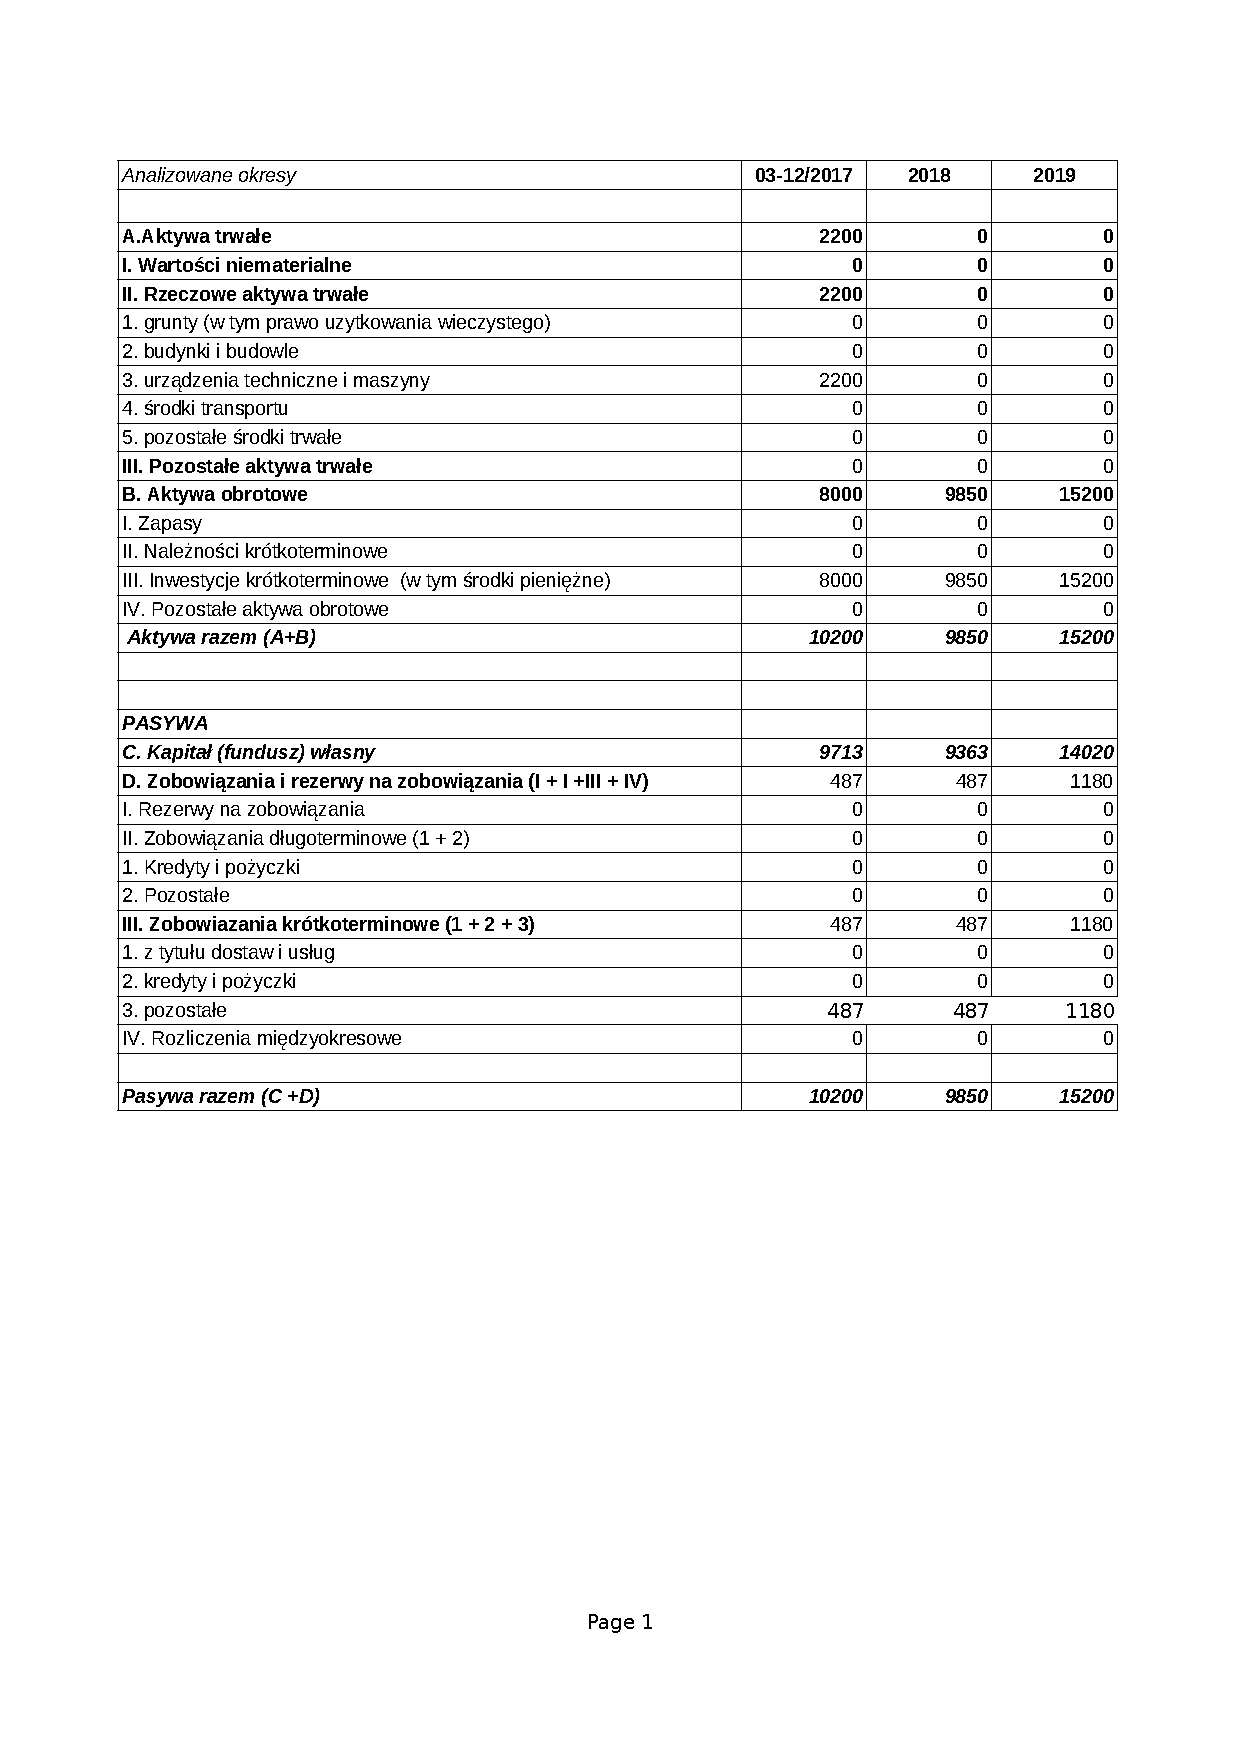
\includepdf[pages={1-},scale=0.9]{bilans.pdf}
	
	\subsubsection{Opis}
		\begin{itemize}
			\item Aktywa trwałe/Rzeczowe aktywa trwałe/urządzenia techniczne i maszyny- kwota 2200 zł dotyczy posiadanego przeze mnie laptopa niezbędnego do prowadzenia sklepu internetowego.
			\item Aktywa obrotowe/Inwestycje krótkoterminowe- kwota 8000 zł odnosi się do posiadanych przeze mnie oszczędności, które przeznaczę na zakup mebli biurowych, reklamę i inne niezbędne rzeczy potrzebne na początku funkcjonowania firmy.
			\item Pasywa/Kapitał własny- kwota 9713 zł to kapital wlasny na pokrycie swoich aktywów.
			\item Pasywa/Zobowiązania krótkoterminowe/Pozostałe- kwota 487 zł to suma składek ZUS z dobrowolnym ubezpieczeniem chorobowym.
			
			
		\end{itemize}	
	
	
	
		



